\section{Introduction}
\label{sec:intro}

\begin{figure*}[!tbh]
%\centering
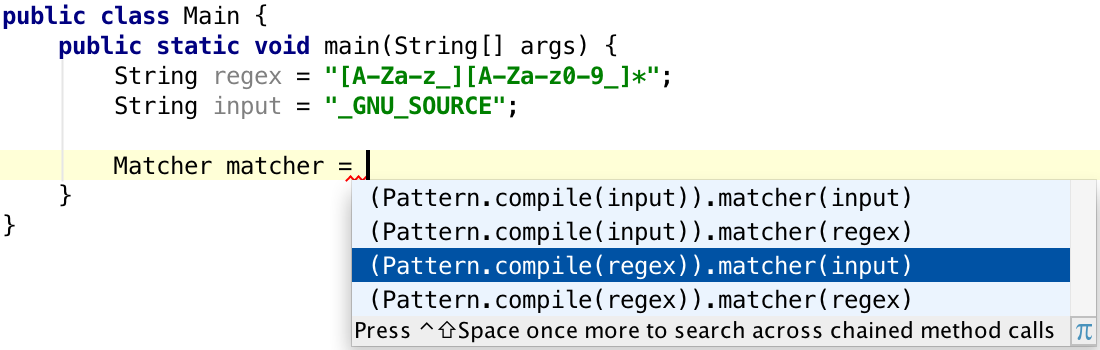
\includegraphics[natwidth=\textwidth]{RegexMatcher.png}
\caption{{\ourTool} suggesting five highest-ranked 
well-typed expressions synthesized from declarations visible at a given program point\label{fig:screenshot1}}
\end{figure*}


Software development provides a high degree of freedom and many different approaches can be adopted for writing code. Still, when writing a program, the developer needs to follow the strict rules determined by the programming language. While coding, the developer often knows the approximate structure of the desired expressions but still may write code that does not compile because some fragments are not well-typed. Such mistakes occur mainly because the developer does not know by heart how to choose and properly combine all the necessary declarations visible from the scope. By the term ``declarations'', we refer to all the elements visible in the scope, such as variables, functions, and class hierarchy declarations. Moreover, modern libraries often evolve into complex application programming interfaces (APIs) that provide a large number of declarations. For this reason it is difficult, if not impossible, to learn the specifics of every declaration and its utilization. In a typical scenario when code does not compile, the compiler outputs an error message with the expression that is at the source of the error. Still, on many occasions the written expression reflects the intended structure of the code. 

As an illustration, a programmer might expect the Java code
\begin{lstlisting}
BufferedReader br = new BufferedReader("file.txt");
\end{lstlisting}
to open a file called ``file.txt". However, this code will not compile since \texttt{BufferedReader} accepts only a \texttt{Reader} interface implementation as an argument. After consulting the documentation, the programmer corrects the previous line to
\begin{lstlisting}
BufferedReader br = 
   new BufferedReader(new FileReader("file.txt"));
\end{lstlisting}
Mistakes like these are common when exploring a new API, or a new language, since classes are often composed in unintuitive ways. A survey conducted on 157 software engineers at Microsoft \cite{LaToza:2006} revealed that a full $56\%$ admit to spending a large amount of time trying to understand code that other people wrote, and $41\%$ agree that the amount of example code adapted for a production setting is a serious problem. We believe that the time spent perusing the API documentation could be spent actually writing the application-specific parts of the code. 

In this paper we describe a tool, called \ourTool, which automatically repairs code expressions based on the hinted structure of the ill-typed code. \ourTool finds well typed expressions that are as close as possible to the given (potentially) ill-typed expression - we call such an input expression, a {\em backbone} expression. 

Additionally, \ourTool can also be seen as a synthesis tool. It extends the functionality described in \cite{MandelinetALL2005Jungloid, GveroETAL13CompleteCompletionTypesWeights, PerelmanGBG12}. In the light of the program repair, the synthesis aspect of \ourTool can be considered as a repair of the empty expression. A user does not need to provide a backbone expression -- it is sufficient to declare a variable of an arbitrary type. Based on that type \ourTool can synthesize corresponding code fragments. The synthesized code has the given type and it can contain user defined values, as well as methods from the API. 

Our tool can be applied in interactive scenarios like IDE code completion, to rank expressions based on their similarity to ill-typed code. Ideally, the best suggestions will correct the code while preserving its overall structure. Another possible application of the \ourTool algorithm is to provide automated repair as a part of the compilation process.

\ourTool is a tool based on a graph algorithm for synthesizing expressions of a certain type in a programming language. As an algorithm, a synthesis process is generalized to repair ill-typed expressions. We believe that this graph construction will prove to be a useful tool for synthesis and repair in other contexts, as well. \ourTool ranks expressions based on a system of costs that appeal to general principles (eg. the principle of locality), but other contexts might call for different valuation schemes in order to bias the synthesis towards or against certain expressions. For example, one might wish to favor resource acquisition near program entry points, but adjust the costs in the other direction when attempting to synthesize snippets deep inside the class hierarchy.

The research on improving the software development process covers a large number of topics such as an automated program repair \cite{LeGoues:2012:ROI:2330163.2330296,WeiETAL10AutomatedFixingProgramsContracts,PeiETAL11CodebasedAutomatedProgramFixing}, enhancements of compiler messages \cite{Burke87apractical,Hammond198451,Lerner:2007:STM:1250734.1250783}, and providing assistance to developers through code inference \cite{GveroETAL13CompleteCompletionTypesWeights, MandelinetALL2005Jungloid, KneussETAL13SynthesisModuloRecursiveFunctions, KuncakETAL13ExecutingSpecificationsSynthesisConstraintSolvingInvitedTalk, PerelmanGBG12}. As a result, a vast number of tools have been created around a common high-level goal of expediting software development. The manner in which such tools operate can be broadly divided into two categories: (1) as automated processes within the compiler (2) or as development assistants that require a certain level of interaction, usually through an IDE interface. Many of the techniques behind these tools such as parsing error recovery by altering the input \cite{Burke87apractical}, a heuristic search for syntactically correct terms \cite{PerelmanGBG12}, a modification of abstract syntax trees and types \cite{Lerner:2007:STM:1250734.1250783}, and inference of semantically correct code fragments \cite{KneussETAL13SynthesisModuloRecursiveFunctions}, share common insights.

Motivated by the advances in both the theory of programming languages and techniques that are foundations of tools for software development, our approach addresses the problem of code repair from a new perspective, by providing an algorithm that extends existing methods and incorporates new ideas. Our tool goes beyond the existing line of work is three important ways: (1) the algorithm tries to solve more general code repair problems constrained by  the structure of given ill-typed terms, (2) it focuses on repairing programs in as much accurate way as possible, according to the given hint and weight heuristics, while providing useful theoretical guarantees about the utilized repair algorithms, (3) it is suitable for realization as both an interactive and automated software development tool.

The principal contributions of this paper are:
\begin{itemize}\itemsep0pt
	\item An especially-efficient synthesis and repair algorithm. \ourTool outperforms existing tools, sometimes by several orders of magnitude, while still producing high-quality results. From a theoretical standpoint, the \ourTool algorithm is sound and complete.
	\item A practical implementation of this algorithm as an IntelliJ IDEA plugin. The code will be made available on the first author's website.
\end{itemize}
